% !TEX TS-program = xelatex
% !TEX encoding = UTF-8 Unicode
% !Mode:: "TeX:UTF-8"

\documentclass{resume}
\usepackage{graphicx}
\usepackage{tabu}
\usepackage{multirow}
\usepackage{progressbar}
\usepackage{zh_CN-Adobefonts_external} % Simplified Chinese Support using external fonts (./fonts/zh_CN-Adobe/)
% \usepackage{NotoSansSC_external}
% \usepackage{NotoSerifCJKsc_external}
% \usepackage{zh_CN-Adobefonts_internal} % Simplified Chinese Support using system fonts
\usepackage{linespacing_fix} % disable extra space before next section
\usepackage{cite}
\usepackage{fontspec}

\begin{document}
\pagenumbering{gobble} % suppress displaying page number

\Large{
  \begin{tabu}{ c l r }
   \multirow{5}{1in}{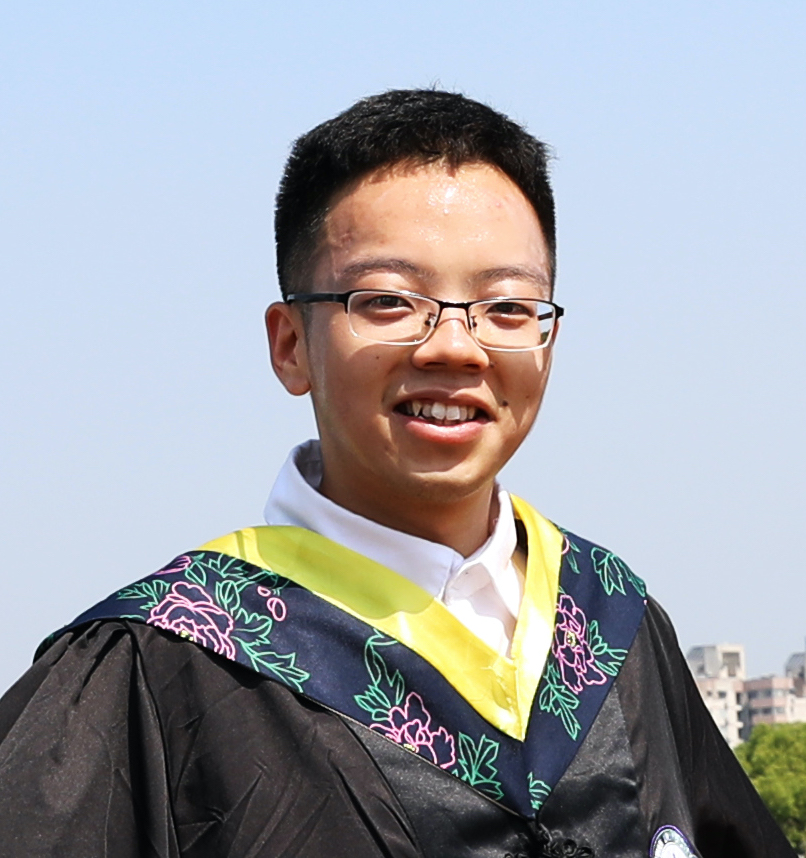
\includegraphics[width=0.95in]{img-me1.jpg}} & \scshape{张雪遥} &  \\
    & \email{zhangxueyao19s@ict.ac.cn} &  \\
    & \phone{(+86) 152-0390-0168} &  \\
    & \faWechat{ xueyao\_98} & \\
    & \github[github.com/RMSnow]{https://github.com/RMSnow} &
    % & \homepage[Xueyao Zhang]{https://www.zhangxueyao.com} & 
  \end{tabu}
}

\section{教育背景}
\datedsubsection{\textbf{中国科学院计算技术研究所},计算机应用技术,学术型硕士}{2019.09 -- 2022.06}
{\small 前瞻实验室,研究方向:大规模社交媒体数据挖掘,导师:曹娟研究员;GPA:3.79 / 4.00}

\datedsubsection{\textbf{武汉大学},软件工程,学士}{2015.09 -- 2019.06}
{\small GPA:3.84 / 4.00,专业排名:4 / 246,英语六级:522}

\section{研究经历}
\datedsubsection{\textit{\textbf{Mining Dual Emotion for Fake News Detection} (Full Paper)}}{2020.04 -- 2021.04}
{\small \role{\textbf{Xueyao Zhang}, Juan Cao, Xirong Li, Qiang Sheng, Lei Zhong, Kai Shu.}{发表于\textit{WWW'2021} \textbf{(CCF-A)};第一作者}
}Brief introduction: xxx.
\begin{itemize}
  \item Implemented xxx feature
  \item Optimized xxx 5\%
  \item xxx
\end{itemize}

% \datedsubsection{\textit{\textbf{Article Reranking by Memory-enhanced Key Sentence Matching for Detecting Previously Fact-checked Claims} (论文在投)}}{2020.09 -- 2021.02}
% {\small \role{Qiang Sheng, Juan Cao, \textbf{Xueyao Zhang}, Xirong Li and Lei Zhong.}{投稿于\textit{ACL'2021};学生第二作者}}

\section{编程技能}
\small
\begin{itemize}
  \item 编程语言:熟练使用Python,熟悉Java,了解C++.
  \item 深度学习框架:PyTorch、Keras.
\end{itemize}

\section{获奖情况}
\begin{itemize}
  \item 中国科学院大学计算机学院三好学生(2020)
  \item 武汉大学优秀学士学位论文(2019)
  \item 武汉大学三好学生、优秀团员、优秀学生干部(2016--2018)
  \item 本科生国家奖学金(2016)
  \item 全国高中生数学联赛一等奖(2014)
\end{itemize}

% \datedsubsection{中国科学院大学计算机学院三好学生}{2020}
% % \datedsubsection{武汉大学优秀学生甲等奖学金}{2018,2017,2016}
% \datedsubsection{武汉大学优秀学士学位论文}{2019}
% \datedsubsection{武汉大学三好学生、优秀团员、优秀学生干部}{2016 -- 2018}
% % \datedsubsection{武汉大学优秀团员}{2017}
% % \datedsubsection{武汉大学优秀学生干部}{2016}
% \datedsubsection{本科生国家奖学金}{2016}
% \datedsubsection{全国高中生数学联赛一等奖}{2014}

\end{document}
